\documentclass[superscriptaddress,showpacs,reprint]{revtex4-1}
\usepackage{hyperref}
\usepackage{epsfig}
\usepackage{bm}
\usepackage{graphicx}
\usepackage{epstopdf}
\usepackage{physics}
\usepackage{siunitx}
\usepackage[super]{nth}
%\usepackage{polyglossia}
%\usepackage{unicode-math}
\usepackage{color}
\usepackage{fontspec}
\usepackage{subfig}
%\usepackage[affil-it]{authblk}
%\usepackage{fixltx2e}
%\usepackage{dblfloatfix}
\hypersetup{
    colorlinks=true,       % false: boxed links; true: colored links
    linkcolor=cyan,          % color of internal links
    citecolor=magenta,        % color of links to bibliography
    filecolor=magenta,      % color of file links
    urlcolor=cyan,           % color of external links
    runcolor=cyan
}
\newcommand{\figurewidth}{0.8 \columnwidth}
\newcommand{\beqarr}{\begin{eqnarray}}
\newcommand{\eeqarr}{\end{eqnarray}}
\newcommand{\beq}{\begin{equation}}
\newcommand{\eeq}{\end{equation}}
\newcommand{\e}{{\text e}}
\newcommand{\rmd}{{\text d}}
\newcommand{\mc}{\mathcal}
\newcommand{\byJJ}[1]{{\textcolor{red}{#1}}}
\newcommand{\byDL}[1]{{\textcolor{blue}{#1}}}
\newcommand{\byAM}[1]{{\textcolor{green}{#1}}}
\newcommand{\byMS}[1]{{\textcolor{orange}{#1}}}
\newcommand{\GeV}{\giga\electronvolt}
\newcommand{\TeV}{\tera\electronvolt}
\usepackage{amsmath}
\usepackage{mathtools}
%\defaultfontfeatures{Ligatures=TeX,Mapping=tex-text} 
%\setmainfont[Mapping=tex-text]{Palatino}
%\setsansfont[Scale=MatchLowercase,Mapping=tex-text]{Gill Sans}
%\setmonofont[Scale=MatchLowercase]{Andale Mono}


\begin{document}
\title{Embedding fully connected problems in graphs capable on graphs with known error suppression strategies}
\author{Joshua Job, Itay Hen}
\maketitle

Recently, a proposal for representing fully connected problem graphs with purely local connections by Wolfgang Lechner, Philipp Hauke, and Peter Zoller (draft) has gained attention, largely because it is a different embedding than Vicki Choi's standard embedding for the Chimera graph \cite{Choi1,Choi2}. It is also hypothesized to have certain nice properties regarding decoding and resilience to certain sorts of errors.

Based on this, and statements by D-Wave Systems regarding their interest in potential new architectures, one may seek ways to embed fully connected problems into other architectures than Chimera. The most natural alternative graphs are the two graphs for which error suppression techniques are already known and implementable on current and next-generation quantum annealing hardware: the Pudenz and Paz QAC-ME graphs \cite{PAL:14,Vinci:2015um}. The Pudenz code graph can be solved exactly in $2^{L+1}$ steps for an $L\cross L$ unit cell graph, while the Paz graph requires $4^{L+1}$ steps. The Pudenz code graph (KPG) is essentially the Paz code graph (GPG) where one removes all the connections across the rows in one layer and all the connections across columns in the other. A plot of the GPG is shown in Figure \ref{fig:gpg}
\section{Motivation and Procedure}
If one strongly ferromagnetically binds together the qubits within each row of one layer of the 2D square lattice in the GPG (or the layer in which rows are connected in the KPG) to form logical qubits, while also binding together the qubits within the columns of the other layer, one can readily see the resulting logical graph will be a complete bipartite graph \ref{fig:kgp2bipartite}. Indeed, this is exactly how D-Wave constructs its $K_{4,4}$ unit cells, except that instead of multiple qubits bound together by couplers to form a line, they use qubits which form very long, thin loops, but in the same crosshatch pattern.

To construct a fully connected logical graph, one simply binds together a logical qubit in one layer of the bipartite graph with a logical qubit from the other layer \ref{fig:full2bipartite}. The resulting logical qubit will have connections to every other qubit. Doing this for all pairs results in a fully connected graph, where each logical qubit is formed by a chain or simple tree, and all encoded chains interact with the other chains at two locations. For an $L\cross L$ GPG/KPG graph, one thus encodes $L$ logical qubits, using $2L^2$ physical qubits to do so. This embedding is actually the result of the Choi embedding procedure, applied to qubits which have degree of at most $3$ instead of degree $6$, as in Chimera (though it was discovered independently by the author).

\section{Properties}

This embedding has certain nice properties. One is that there is are simple combinatorial degrees of freedom, over which one can trivially perform gauge averaging to improve performance --- namely, that when moving from the bipartite graph to the fully connected graph, one has complete freedom over which (row,column) pairs one assigns to form a chain, and which physical chain one assigns to which logical label. One chooses from any of the $L$ bits in the first layer, and pairs it with any of the $L$ bits in the second layer, then any of the $L-1$ with any of the remaining $L-1$, and so on, yielding a total of $L!^2$ possible chains with $L!$ labelings, yielding a total of $L!^3$ embeddings into the physical problem space due to geometric considerations alone. 

 This embedding is also implementable directly on a subset of the connections on current D-Wave hardware, and that one can use either the Pudenz or Paz QAC-ME techniques on current hardware to improve performance. The lower degree compared to Chimera enables a simpler tile (simply two elongated qubits overlapping) thus reducing crosstalk effects and coupler noise on each physical qubit, as there are fewer couplers on each qubit and the couplers and qubits are farther apart. Of course, this does not include QAC-ME techniques, but it may be an interesting avenue to investigate from the perspective of hardware designers.

\section{Next steps and conclusion}
Next steps are to consider performance in simulation of this embedding in simulated annealing and HFS and compare to similar results for Chimera. Ideally, tests on D-Wave itself could be performed, to detect what effects QAC-ME techniques have on performance, though due to the small values of $L$ involved in the KPG/GPG graphs (no more than $12$ on a D-Wave 2X machine), it is unlikely one will be able to see much improvement in performance without significantly reducing the overall strength of the Hamiltonian as a ``poor man's temperature switch'', as was done in  \cite{PAL:14,Vinci:2015um}. One important outstanding mathematical question is if there is a way to more efficiently embed a problem into the GPG, as one may expect from it's greater intrinsic complexity, since it's intrinsic complexity seems to correspond to twice as many bits as that of KPG for a fixed number of unit cells. Work is continuing in that direction.

Embedding fully connected problems in either a) simpler graphs than Chimera with reduced noise and without loss of qubit efficiency/chain compactness or b) graphs on which we know how to perform some manner of error suppression or correction is likely to be highly valuable in solving real-world problems on quantum annealers, and is worthy of further investigation. 

\begin{figure}[hbt]
  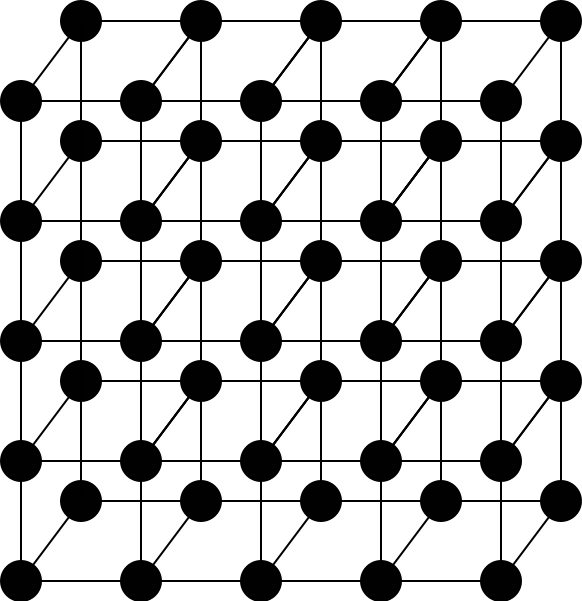
\includegraphics[width=\textwidth/2]{2lsl}
  \caption{The Paz code logical graph for a $5\cross 5$ unit cell graph.}
  \label{fig:gpg}
\end{figure}

\begin{figure}[hbt]
  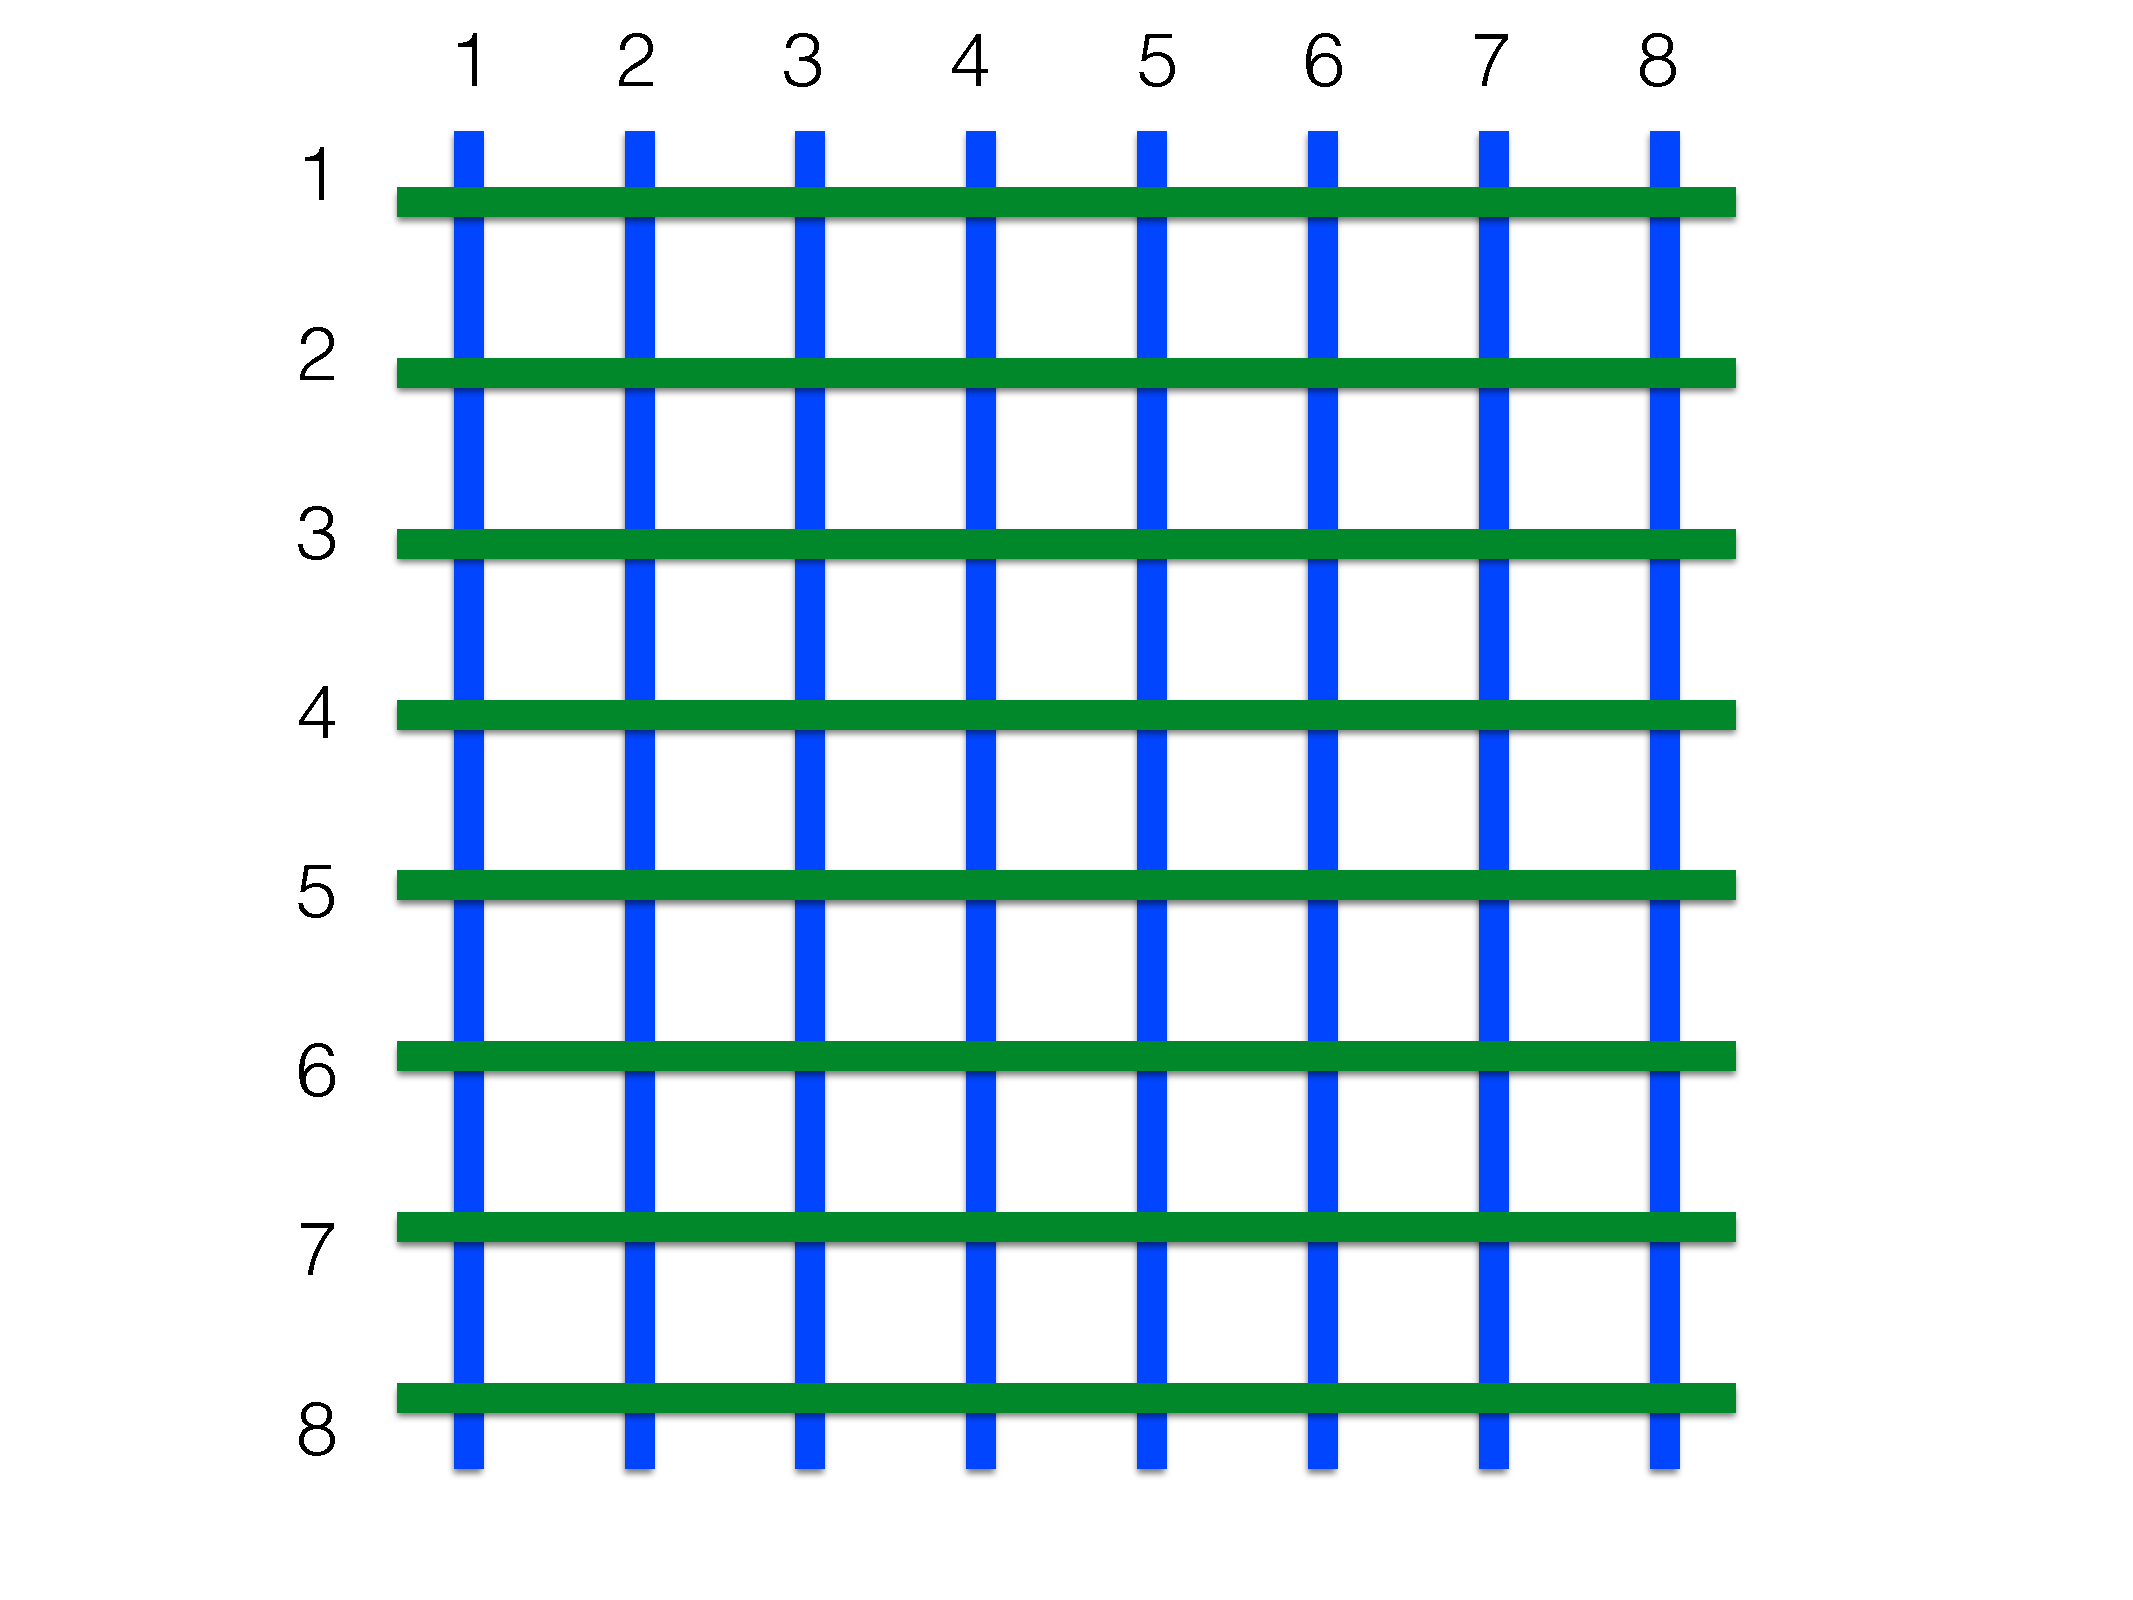
\includegraphics[width=\textwidth/2]{rowsncolumns}
  \caption{The KGP graph, where two nodes are implicitly located at the crossings of the blue and green lines, and can be named by their coordinate. $(B,2,6)$ would denote the node in the blue layer in the 2nd row and 6th column and connects only to blue layer qubits above and below it, while there is another node $(G,2,6)$ at the same grid point in the green layer which is connected to $(B,2,6)$ and also to the nodes in the green layer to the left and right. Each green or blue line denotes a set of physical qubits which are strongly ferromagnetically bound together, thus forming a single logical qubit. It is obvious that this forms a complete bipartite graph in the logical space, by inspection. For an $L$ node complete bipartite graph, one needs an $LxL$ unit cell KGP graph.}
  \label{fig:kgp2bipartite}
\end{figure}

\begin{figure}[hbt]
  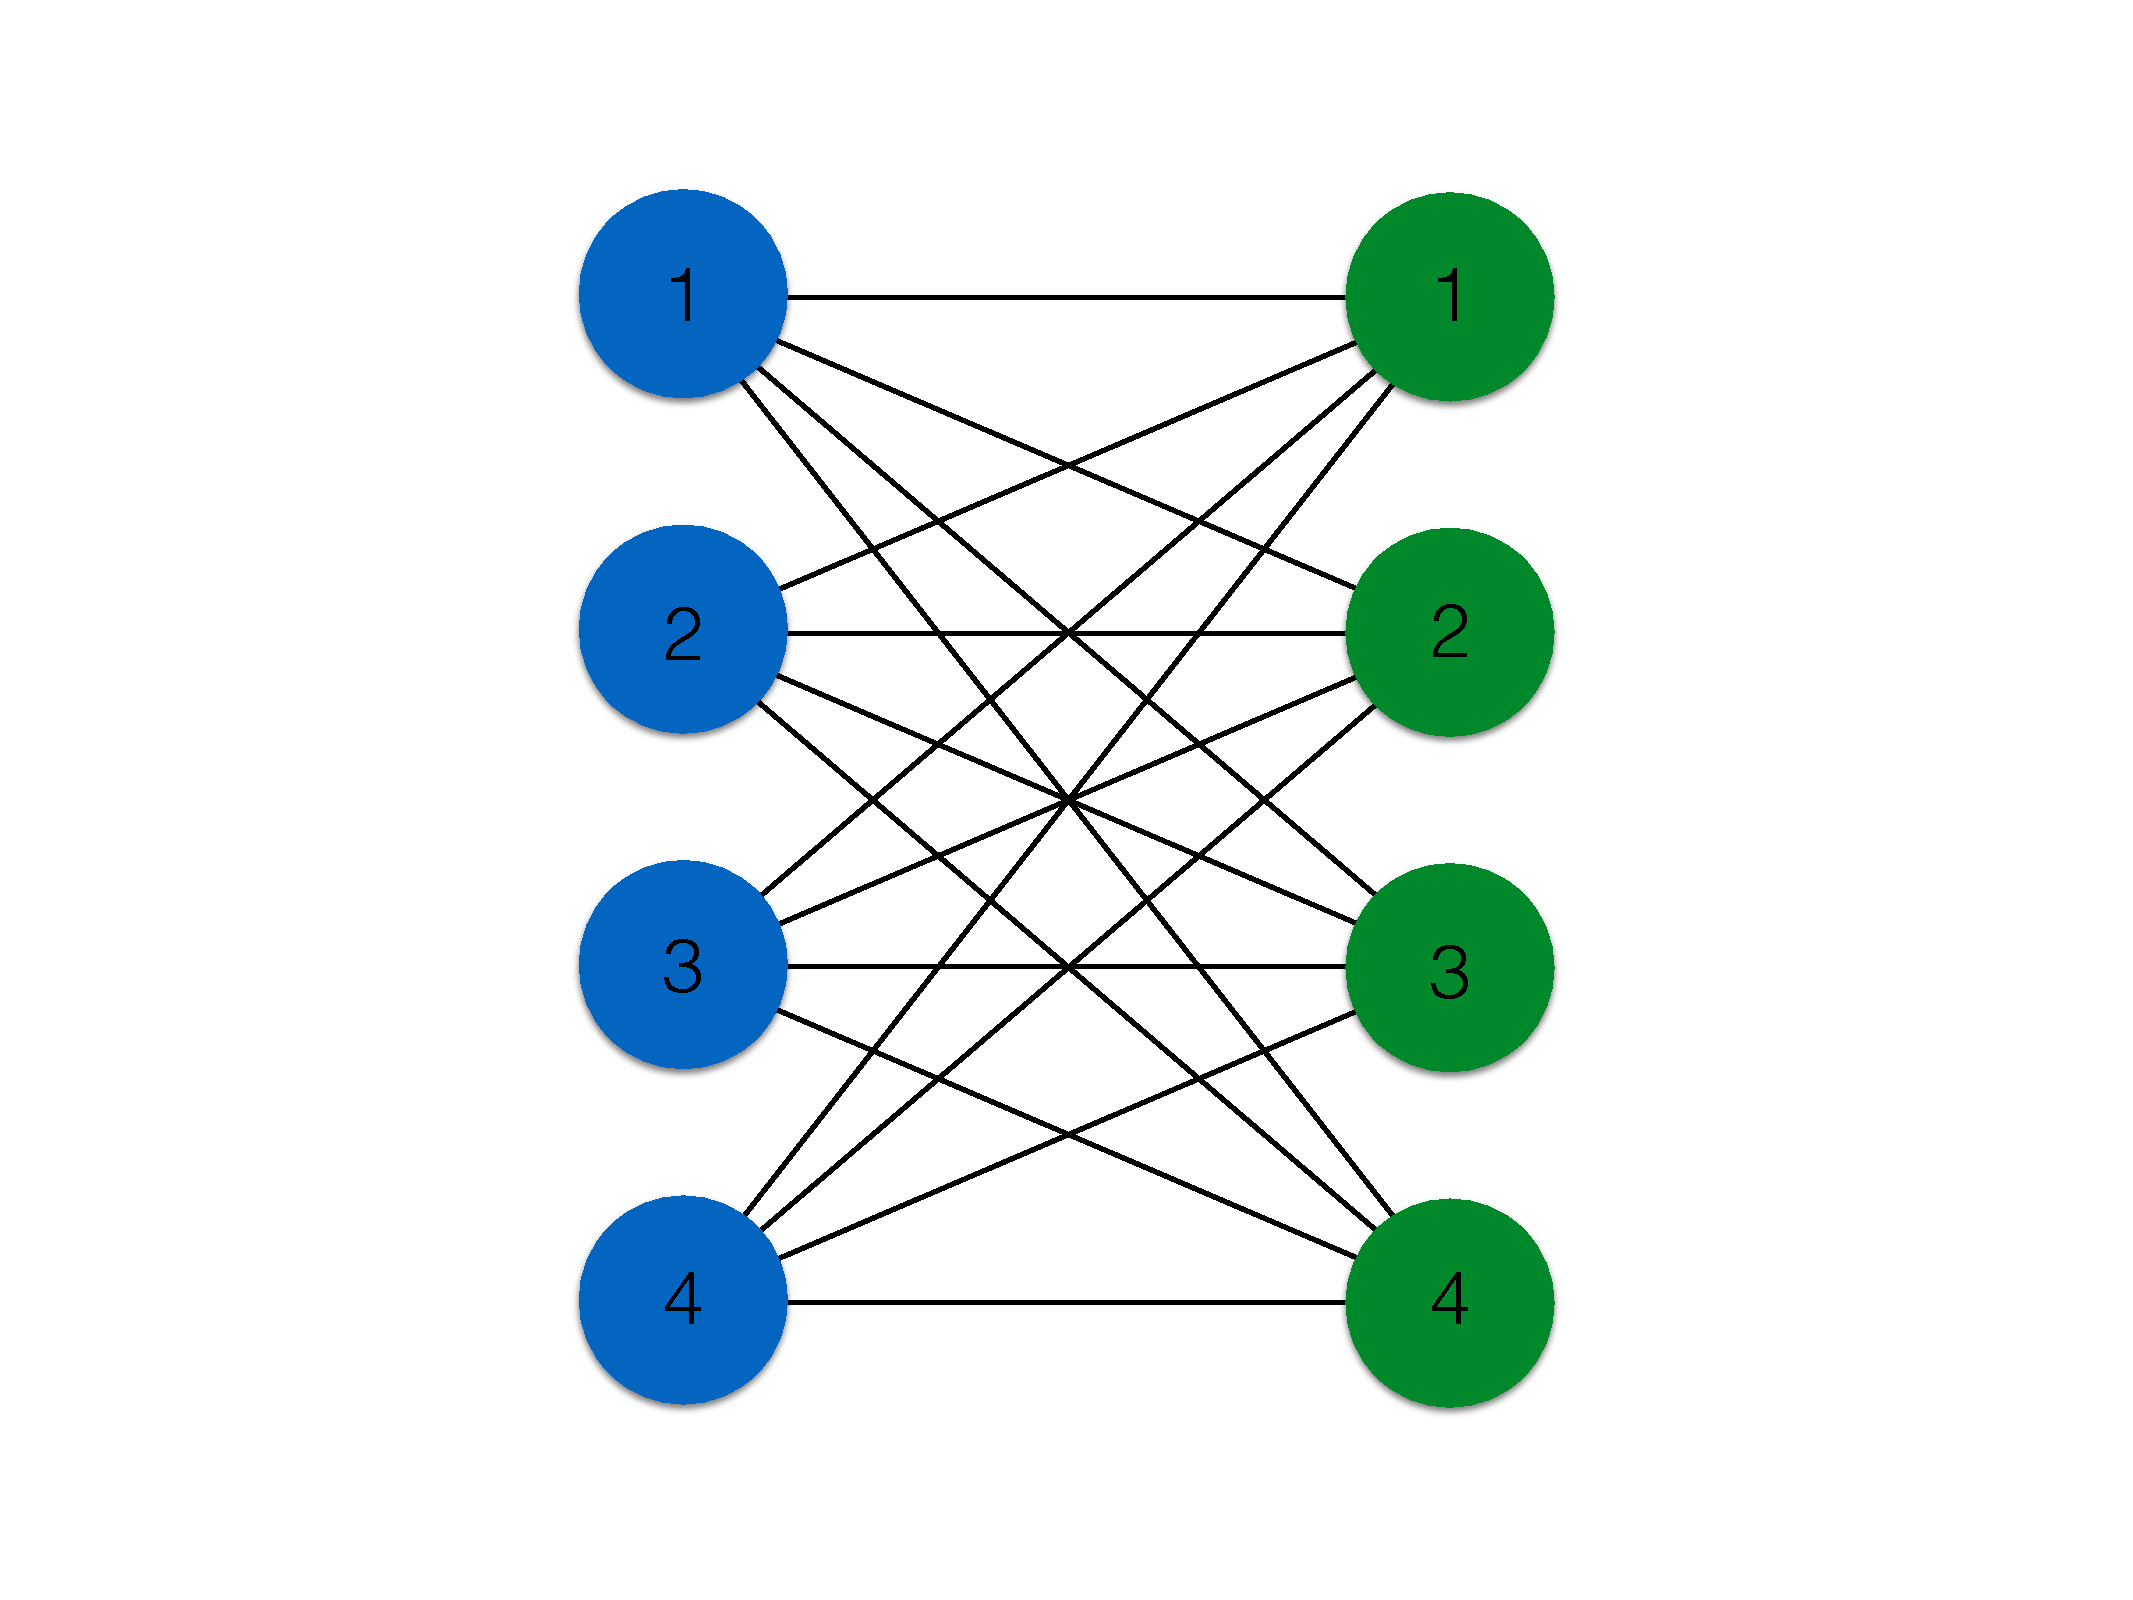
\includegraphics[width=\textwidth/2]{bipartitetofull}
  \caption{Here, the blue nodes denote the blue lines/chains from Figure \ref{fig:kgp2bipartite}, and the green nodes the green lines/chains from the same. Nodes with matching numbers will be ferromagnetically bound together to form a single logical qubit in order to form the complete graph. Since it is complete and bipartite, coupling all pairs of two nodes, one in each layer, will create a fully connected logical graph with half as many nodes. This can be verified by inspection. When concatenating this with the mapping from KGP to a complete bipartite graph, one finds you can map a $K_L$ to an $LxL$ unit cell KGP graph at a cost of $2L$ embedded nodes per logical node.}
  \label{fig:bipartite2full}
\end{figure}

\bibliography{\string~/Dropbox/nature-QA-higgs/v0851/refs}

\end{document}
